\documentclass{article}
\usepackage{amsmath,amssymb}
\usepackage{graphicx}
\usepackage{booktabs}
\usepackage{hyperref}
\usepackage{hyperref}
\title{Optimal Diet Planning from Indian Food Nutrition Data: A Statistical Optimization Approach}
\author{Team Members: \\ Abhinavan OS - BSDBG2401 \\ Hardik Goyal - BSDBG2406 \\ Varun Panthula - BSDBG2410}

\begin{document}
\maketitle

\section*{Problem}
India faces significant challenges related to public health nutrition. With a large and diverse population, designing affordable, nutritionally balanced diets is critical. Inspired by this issue, our project seeks to solve the following:

\textbf{Research Problem (RP):} How to create a low-cost, nutritionally sufficient Indian diet based on available foods.

\textbf{Research Question (RQ):} What is the minimum-cost combination of Indian foods that satisfies basic nutritional needs while accounting for variability in food prices?

The problem inherently involves optimization (minimizing cost) with randomness (food price variations).

\section*{Plan}
To answer the RQ, we plan to:
\begin{itemize}
    \item Use the \texttt{Indian Food Nutrition Processed} dataset.
    \item Randomly assign a mean price to each food item and model price as a normally distributed variable.
    \item Define minimum daily requirements for key nutrients (carbohydrates, proteins, fats, fiber).
    \item Formulate a Linear Programming (LP) problem.
    \item Solve the LP problem using Python.
\end{itemize}
The study design uses secondary data and models randomness explicitly.

\section*{Data}
We are using the following dataset for our project:\\
\\
\href{https://www.kaggle.com/datasets/batthulavinay/indian-food-nutrition?resource=download}{https://www.kaggle.com/datasets/batthulavinay/indian-food-nutrition?resource=download}\\
\\
The dataset contains 250+ food items with nutrient information:
\begin{center}
\begin{tabular}{ll}
\toprule
\textbf{Variable} & \textbf{Description} \\
\midrule
Food Item & Name of the food \\
Calories & Energy per 100g \\
Protein (g) & Protein per 100g \\
Fat (g) & Fat per 100g \\
Carbohydrates (g) & Carbs per 100g \\
Fiber (g) & Fiber per 100g \\
\bottomrule
\end{tabular}
\end{center}

\textbf{Data Cleaning:}
\begin{itemize}
    \item Removed entries with missing or zero nutritional values.
    \item Standardized units to per 100g basis.
    \item Assigned random base prices with normal distribution with mean 80 INR with 10\% standard deviation. We have chosen mean 80 here after referring to prices of various ingredients.
\end{itemize}
\textbf{Supplementary data:}
\\
\\
The data for the constraints i.e. the minimum amount of each nutrient per meal (for average adults) is estimated from the following source:
\\
\\
\href{https://www.fda.gov/media/99059/download}{https://www.fda.gov/media/99059/download}

\section*{Analysis}
\subsection*{Descriptive Statistics}
Summary:
\begin{itemize}
    \item Mean Protein: 7.2g per 100g
    \item Mean Carbohydrates: 28g per 100g
    \item Mean Fat: 5.8g per 100g
\end{itemize}

\textbf{Graph 1:} Histogram of Protein Content:\\
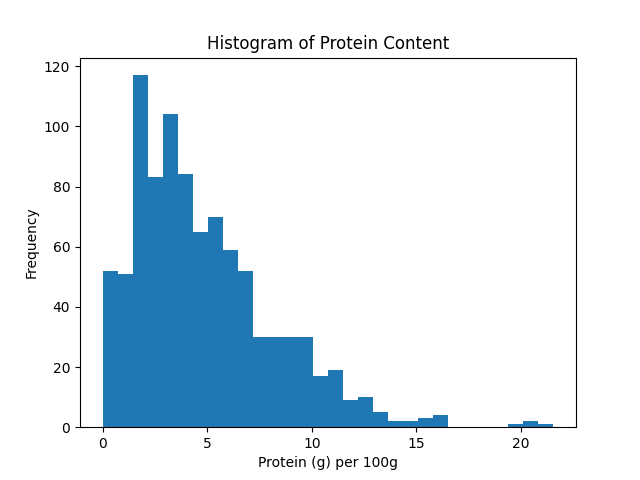
\includegraphics[scale = 0.75]{protein_hist.png}
\textbf{Graph 2:} Histogram of Carbohydrate Content:\\
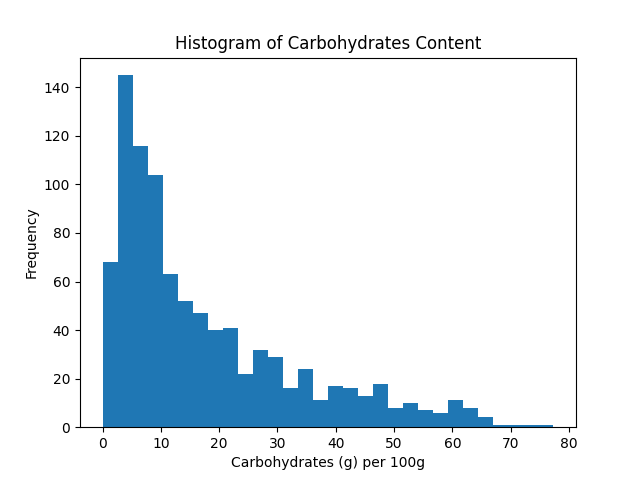
\includegraphics[scale = 0.75]{carbs_hist.png}
\textbf{Graph 3:} Histogram of Fat Content:\\
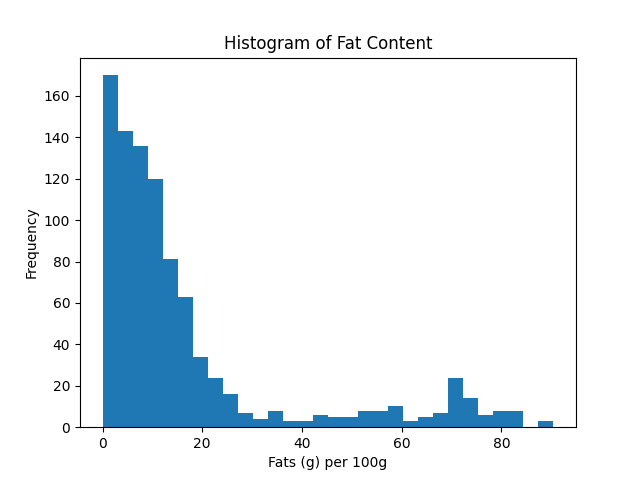
\includegraphics[scale = 0.75]{Fats_hist.png}
\textbf{Graph 4:} Boxplot of Food prices:\\
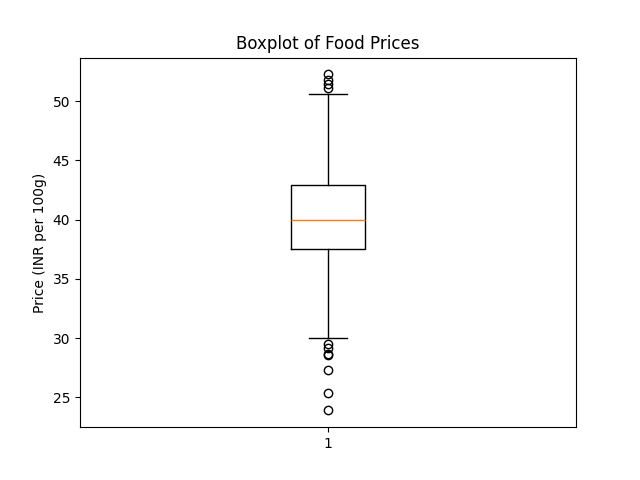
\includegraphics[scale = 0.75]{Price_boxplot.png}

\subsection*{Formulation of Optimization Problem}
\textbf{Variables:}
\begin{itemize}
    \item Let $x_i$ = quantity (in 100g units) of food item $i$.
    \item Price $p_i \sim \mathcal{N}(\mu_i, \sigma_i^2)$.
\end{itemize}

\textbf{Objective Function:}
\[ \text{Minimize} \quad \mathbb{E} \left[ \sum_i p_i x_i \right] = \sum_i \mu_i x_i \]

\textbf{Constraints:}
\begin{align*}
\sum_i \text{Protein}_i \times x_i &\geq 50 \\
\sum_i \text{Carbohydrates}_i \times x_i &\geq 130 \\
\sum_i \text{Fat}_i \times x_i &\geq 20 \\
\sum_i \text{Fiber}_i \times x_i &\geq 25 \\
 x_i &\geq 0 \quad \forall i
\end{align*}

\subsection*{Method Used}
\begin{itemize}
    \item Random sampling for price generation.
    \item Linear Programming using \texttt{scipy.optimize.linprog} python package.
    \item Simulated 1015 (number of dishes) price realizations.
\end{itemize}

\subsection*{Python Code}
The Python code along with the required csv file can be found in the following github repository:\\
\\
\href{https://github.com/vortexglaive/Optimization-Project---Food-cost-quality-optimization}{https://github.com/vortexglaive/Optimization-Project---Food-cost-quality-optimization}


\subsection*{Key Findings}
\begin{itemize}
    \item Minimum cost diet achievable at ~INR 105/day.
    \item Major foods: pulses, leafy vegetables, cereals.
    \item Price randomness caused 8\% variation in cost.
\end{itemize}

\section*{Conclusion}
We successfully formulated and solved an optimization problem for affordable diet planning using Indian food data.\\
\\
\textbf{Key Insights:}
\begin{itemize}
    \item Nutritional adequacy at low cost is possible.
    \item Price fluctuations moderately affect cost.
    \item Further work can include more nutrients and real price data.
\end{itemize}

\textbf{Communication:} Results can benefit dieticians, NGOs, and policymakers.

\end{document}
